% Provenance (never printed): see sources/outline_sources.md (Year 3: elastic waves
% recalled from the physics books; rays in a spherical Earth; travel-time tables;
% surface waves and dispersion; normal modes, told; linear inverse problems and
% seismic tomography). Brief: sources/book5/BRIEFS.md, ch. 1. Curves from
% figdata/bachelor-3/ray_tracing.py, love_dispersion.py, tomo_checkerboard.py;
% exercise and problem values in the Book 5 scratch calculator calc/ch01.py.
\chapter{Seismologi dan Pencitraan Bumi}\label{ch:b3:seismology-imaging}

Pada 22 Mei 1960, pukul 19.11 waktu universal, gempa bumi terbesar yang tercatat sejak
1900 memutus zona subduksi di lepas pantai Chile selatan, dengan magnitudo 9.5.
% ledger: usgs5:chile1960
Gelombang P-nya mencapai stasiun di sisi seberang planet sekitar dua puluh menit
kemudian; gelombang permukaannya mengelilingi Bumi beberapa kali; dan selama berhari-hari
sesudahnya instrumen paling lambat merekam seluruh Bumi bergetar dengan
periode mendekati satu jam, seperti lonceng yang dipukul. Setiap sinyal ini membawa
informasi tentang batuan yang dilaluinya. Dari waktu tiba jutaan
gelombang seperti itu yang tercatat di ribuan stasiun, para seismolog telah membangun tidak hanya
model berlapis Bumi yang diulas di bawah, tetapi juga citra tiga dimensi
mantel, tempat lempengan yang tenggelam dan plume mantel yang naik tampak sebagai daerah
tempat gelombang merambat sedikit lebih cepat atau lebih lambat daripada rata-rata. Bab ini menunjukkan caranya:
bagaimana sinar merambat melalui Bumi berbentuk bola, bagaimana gelombang permukaan
menyelidiki kerak dan mantel melalui dispersinya, bagaimana osilasi bebas seluruh
planet dideskripsikan, dan bagaimana beberapa ribu waktu tempuh diubah menjadi
gambaran dengan menyelesaikan \omterm{def:b3:seismology-imaging:inverse}{masalah invers} linier.

\begin{recall}
Dalam padatan elastis isotrop dua jenis gelombang badan merambat: gelombang P, dengan
laju $\alpha = \sqrt{(K + \tfrac43\mu)/\rho}$, dan gelombang S, pada
$\beta = \sqrt{\mu/\rho}$, dengan $K$ dan $\mu$ masing-masing modulus bulk dan modulus geser
dan $\rho$ massa jenis; gelombang S tidak menembus cairan (volume Tahun 3 buku fisika,
pada bab elastisitas kontinum). Gelombang yang laju fasenya bergantung
pada frekuensinya bersifat dispersif; energinya merambat dengan laju
grup $U = \mathrm d\omega/\mathrm dk$ (volume Tahun 2 buku fisika, tentang
gelombang). Benda elastis terbatas bergetar bebas dalam himpunan diskret mode normal
(volume yang sama). Jarak episentral $\Delta$ sebuah stasiun adalah sudut
di pusat Bumi antara episentrum dan stasiun; kurva waktu tempuh
memberikan waktu tiba pertama terhadap $\Delta$, dan inti menghasilkan
zona bayangan bagi gelombang P langsung (Buku 2, kelas 11). Model acuan Bumi,
diskontinuitas seismik, dan gelombang kepala telah dibahas di volume Tahun 1,
pada bab tentang Bumi berlapis. Kuadrat terkecil dan hukum galat Gauss
dibahas di buku matematika.
\end{recall}

\section{Sinar pada Bumi berbentuk bola}

Muka gelombang seismik, jauh dari sumbernya dan di dalam medium yang sifatnya
berubah perlahan dalam satu panjang gelombang, dapat diikuti dengan sinarnya: kurva-kurva
yang di mana-mana tegak lurus pada muka gelombang, dan sepanjang kurva itulah energi merambat. Dalam
medium berlaju seragam sinarnya lurus; di tempat laju berubah, sinar
membelok menurut hukum Snell tentang refraksi. Di Bumi laju terutama bergantung pada
kedalaman, sehingga model pertama simetris bola: laju $v(r)$ gelombang
yang ditinjau (P atau S) merupakan fungsi jari-jari $r$ saja.

\begin{theorem}[Hukum Snell pada Bumi berbentuk bola]\label{thm:b3:seismology-imaging:snell}
Dalam Bumi yang simetris bola dengan laju gelombang $v(r)$, misalkan $i$ adalah sudut
antara sinar dan jari-jari di titik berjari-jari $r$. Sepanjang sinar,
\[
  \frac{r\sin i}{v(r)} = p
\]
bernilai konstan.
\end{theorem}

\begin{proof}
Gantikan Bumi dengan kulit-kulit konsentris tipis, masing-masing berlaju seragam. Di dalam
kulit, sinar berupa garis lurus; garis lurus pada jarak $d$ dari
pusat memotong bola berjari-jari $r$ pada sudut $i$ dengan
$r\sin i = d$ (segitiga siku-siku yang dibentuk oleh pusat, kaki tegak lurus, dan
titik itu), sehingga $r\sin i$ sama di bagian atas maupun di
bagian bawah kulit. Pada batas berjari-jari $r$ antara dua kulit dengan laju
$v_1$ dan $v_2$, hukum Snell memberikan $\sin i_1/v_1 = \sin i_2/v_2$, sehingga
$r\sin i/v$ kontinu melintasi batas itu. Di dalam kulit $v$ konstan dan
$r\sin i$ konstan, sehingga $r\sin i/v$ juga konstan di sana. Dengan demikian
ia konstan sepanjang sinar; dengan membiarkan ketebalan kulit menuju
nol, diperoleh hasil untuk $v(r)$ yang kontinu.
\end{proof}

\begin{definition}[Parameter sinar, titik balik]\label{def:b3:seismology-imaging:ray-parameter}
Konstanta $p = r\sin i/v(r)$ suatu sinar pada Bumi yang simetris bola disebut
\emph{parameter sinar}\index{parameter sinar}, dalam detik per radian. Pada
permukaan, $p = R\sin i_0/v_0$, dengan $i_0$ sudut keberangkatan dan $v_0$
laju di permukaan. Titik tempat sinar mendatar ($i = \ang{90}$)
disebut \emph{titik balik}\index{titik balik},
pada jari-jari $r_t$ yang memenuhi
\[
  \frac{r_t}{v(r_t)} = p .
\]
Di bawah titik itu sinar naik kembali, simetris terhadap jari-jari yang melalui
titik balik.
\end{definition}

Tulis $\eta(r) = r/v(r)$. Sinar dengan parameter $p$ hanya dapat ada di tempat
$\eta \ge p$, karena $\sin i = p/\eta \le 1$. Jika $\eta$ berkurang terhadap kedalaman, seperti
yang terjadi di sebagian besar mantel, setiap sinar berbalik pada kedalaman tempat $\eta$
telah turun ke $p$, dan sinar yang berangkat lebih curam (nilai $p$ lebih kecil) berbalik lebih dalam.
Di tempat $\eta$ \emph{bertambah} terhadap kedalaman, karena laju turun tajam
(hal ini terjadi di batas inti--mantel, tempat laju gelombang P turun dari
13.7 hingga \qty{8.0}{km.s^{-1}}), % ledger: ak135:cmb
tidak ada sinar yang dapat berbalik: sinar dibelokkan ke bawah, melintasi lapisan, lalu muncul jauh.
Lompatan semacam itu menghasilkan zona bayangan di permukaan.

\begin{omfigure}
\begin{tikzpicture}[font=\small, x=1.6cm, y=1.6cm]
% concentric shells, centre O at (0,-9) (outside the picture); ray computed by
% Snell's law for v = 1, 1.35, 1.68 and a take-off angle of 30 deg
% (scratch calc/shells_fig.py)
\coordinate (O) at (0,-9);
\fill[blue!6] ($(O)+(62:9)$) arc (62:118:9) -- ($(O)+(118:8.4)$) arc (118:62:8.4) -- cycle;
\fill[blue!12] ($(O)+(62:8.4)$) arc (62:118:8.4) -- ($(O)+(118:7.8)$) arc (118:62:7.8) -- cycle;
\fill[blue!18] ($(O)+(62:7.8)$) arc (62:118:7.8) -- ($(O)+(118:7.0)$) arc (118:62:7.0) -- cycle;
\draw[thick] ($(O)+(62:9)$) arc (62:118:9);
\foreach \r in {8.4, 7.8} {\draw[gray] ($(O)+(62:\r)$) arc (62:118:\r);}
\draw[gray, densely dashed] ($(O)+(62:7.0)$) arc (62:118:7.0);
\node[anchor=east] at ($(O)+(118.3:9)$) {$R$};
\node[anchor=east, gray!60!black] at ($(O)+(118.3:8.4)$) {$r_1$};
\node[anchor=east, gray!60!black] at ($(O)+(118.3:7.8)$) {$r_2$};
\node[blue!60!black] at ($(O)+(64:8.7)$) {$v_0$};
\node[blue!60!black] at ($(O)+(64:8.1)$) {$v_1$};
\node[blue!60!black] at ($(O)+(64:7.4)$) {$v_2$};
\coordinate (A) at (-3.295,-0.625);
\coordinate (B) at (-2.746,-1.062);
\coordinate (C) at (-1.920,-1.440);
\coordinate (T) at (0,-1.440);
\coordinate (C') at (1.920,-1.440);
\coordinate (B') at (2.746,-1.062);
\coordinate (A') at (3.295,-0.625);
% radii at the source and at the first boundary, towards the centre
\draw[densely dashed] ($(A)!-0.04!(O)$) -- ($(A)!0.12!(O)$);
\draw[densely dashed] ($(B)!-0.04!(O)$) -- ($(B)!0.11!(O)$);
\draw[densely dashed] (T) -- (0,-2.15);
\draw[very thick, red!70!black] (A) -- (B) -- (C) -- (T) -- (C') -- (B') -- (A');
\pic[draw, angle radius=0.75cm, pic text={$i_0$}, angle eccentricity=1.4] {angle = O--A--B};
\pic[draw, angle radius=0.65cm, pic text={$i_1$}, angle eccentricity=1.45] {angle = O--B--C};
\fill (A) circle (2pt) node[above left=1pt] {sumber};
\fill (A') circle (2pt) node[above right=1pt] {stasiun};
\fill[red!70!black] (T) circle (1.6pt);
\node[anchor=north west, red!70!black] at (0.05,-1.47) {titik balik, $r_t/v_2 = p$};
\node[anchor=north, font=\scriptsize] at (0,-2.15) {menuju pusat $O$};
\end{tikzpicture}

\par\smallskip{\small Sinar dalam Bumi yang berbentuk bola, dibagi menjadi kulit-kulit berkecepatan seragam
kecepatan (skematik, tidak sesuai skala). Di setiap kulit sinar berupa garis lurus; pada setiap
batas, sinar dibiaskan menurut hukum Snell, menjauhi jari-jari bila kecepatan
bertambah ke bawah. Besaran $r\sin i/v$ tetap bernilai $p$ sepanjang
sinar; sinar mendatar di \omterm{def:b3:seismology-imaging:ray-parameter}{titik baliknya}, tempat $r/v = p$, dan
naik kembali secara simetris.}
\label{fig:b3:seismology-imaging:shells}
\end{omfigure}

\omterm{def:b3:seismology-imaging:ray-parameter}{Parameter sinar} bukan sekadar tetapan sinar: nilainya dapat dibaca dari
kurva waktu tempuh.

\begin{theorem}[Kemiringan kurva waktu tempuh]\label{thm:b3:seismology-imaging:benndorf}
Misalkan $T(\Delta)$ adalah waktu tempuh sinar dari sumber di permukaan ke
stasiun di permukaan pada jarak episentral $\Delta$ (dalam radian). Maka
\[
  \frac{\mathrm dT}{\mathrm d\Delta} = p ,
\]
yakni \omterm{def:b3:seismology-imaging:ray-parameter}{parameter sinar} yang tiba di $\Delta$.
\end{theorem}

\begin{proof}
Tinjau dua sinar bertetangga dari sumber yang sama, yang tiba di permukaan
di $\Delta$ dan $\Delta + \mathrm d\Delta$, keduanya dengan sudut datang $i_0$
terhadap jari-jari. Muka gelombang yang melalui titik pertama tegak lurus sinar;
sinar kedua masih harus menempuh, setelah melintasi muka gelombang itu, sisi
dari segitiga siku-siku kecil yang hipotenusanya adalah busur $R\,\mathrm d\Delta$ sepanjang
permukaan dan sudut di hadapan sisi itu adalah $i_0$: panjang
$R\,\mathrm d\Delta\,\sin i_0$ dengan kecepatan $v_0$. Oleh karena itu
$\mathrm dT = R\sin i_0\,\mathrm d\Delta/v_0 = p\,\mathrm d\Delta$.
\end{proof}

Teorema ini adalah bentuk bola dari relasi $\mathrm dT/\mathrm dx = 1/c$
antara kemiringan kurva waktu tempuh dan kecepatan semu $c$ sepanjang
permukaan. Kedua fungsi $T(p)$ dan $\Delta(p)$ dapat dituliskan sebagai integral
terhadap profil kecepatan.

\begin{proposition}[Waktu tempuh dan jarak sebagai integral]\label{prop:b3:seismology-imaging:integrals}
Dengan $\eta = r/v(r)$ yang menurun terhadap kedalaman, sinar berparameter $p$ yang berbalik
di $r_t$ mencapai
\[
  \Delta(p) = 2\int_{r_t}^{R}\frac{p\,\mathrm dr}{r\sqrt{\eta^2 - p^2}},
  \qquad
  T(p) = 2\int_{r_t}^{R}\frac{\eta^2\,\mathrm dr}{r\sqrt{\eta^2 - p^2}},
\]
dan waktu intersep $\tau(p) = T - p\Delta$ adalah
$\tau(p) = 2\int_{r_t}^{R}\sqrt{\eta^2 - p^2}\,\mathrm dr/r$.
\end{proposition}

\begin{proof}
Sepanjang elemen sinar dengan panjang $\mathrm ds$, jari-jari berubah sebesar
$\mathrm dr = \cos i\,\mathrm ds$ dan sudut di pusat sebesar
$\mathrm d\Delta = \sin i\,\mathrm ds/r$, sehingga $\mathrm d\Delta = \tan i\,\mathrm dr/r$.
Dengan $\sin i = p/\eta$, $\tan i = p/\sqrt{\eta^2 - p^2}$, yang memberikan integral pertama
untuk paruh menurun; paruh naik serupa. Waktu tempuhnya adalah
$\mathrm dT = \mathrm ds/v = \mathrm dr/(v\cos i)$, dan $1/v = \eta/r$,
$1/\cos i = \eta/\sqrt{\eta^2 - p^2}$. Akhirnya $T - p\Delta$ memiliki integran
$(\eta^2 - p^2)/(r\sqrt{\eta^2 - p^2})$.
\end{proof}

Integral-integral ini adalah cara \omterm{def:b3:seismology-imaging:tables}{tabel waktu tempuh} dihitung dari sebuah model. Skrip
penelusuran sinar bab ini melakukan penjumlahan yang sama pada kulit 2-km dari
model acuan PREM, % ledger: data:prem
dan memeriksanya dengan dua cara: dalam bola berkecepatan seragam, tempat sinar berupa
tali busur dan $T = 2R\sin(\Delta/2)/v$ secara tepat (latihan 5), serta terhadap
\cref{thm:b3:seismology-imaging:benndorf}, yang tidak dipakainya.

\begin{omfigure}
\begin{tikzpicture}
\begin{axis}[axis equal image, hide axis, width=0.66\linewidth,
  xmin=-1500, xmax=6700, ymin=-6700, ymax=6700, clip=false]
\addplot[draw=none, fill=gray!8, domain=0:360, samples=181] ({6371*cos(x)},{6371*sin(x)});
\addplot[black, thick, domain=0:360, samples=181] ({6371*cos(x)},{6371*sin(x)});
\addplot[orange!70!black, fill=orange!12, domain=0:360, samples=181] ({3480*cos(x)},{3480*sin(x)});
\addplot[orange!80!black, fill=orange!35, domain=0:360, samples=121] ({1221.5*cos(x)},{1221.5*sin(x)});
\addplot[blue!70!black, unbounded coords=jump] table[x=x, y=y] {figdata/out/bachelor-3-ray_tracing-rays-mantle.dat};
\addplot[red!70!black, unbounded coords=jump] table[x=x, y=y] {figdata/out/bachelor-3-ray_tracing-rays-core.dat};
% shadow zone for direct P, from 98.5 deg to the caustic B at 143.8 deg
\addplot[gray!60!black, line width=3pt, opacity=0.5, domain=98.5:143.8, samples=40]
  ({6371*sin(x)},{6371*cos(x)});
\fill (axis cs:0,6371) circle (2.2pt);
\node[anchor=south] at (axis cs:0,6371) {\small sumber};
\node[anchor=west, font=\small] at (axis cs:{6371*sin(120)+150},{6371*cos(120)}) {zona bayangan};
\node[anchor=west, font=\scriptsize] at (axis cs:{6371*sin(98.5)+120},{6371*cos(98.5)}) {\ang{98.5}};
\node[anchor=west, font=\scriptsize] at (axis cs:{6371*sin(143.8)+120},{6371*cos(143.8)}) {\ang{143.8}};
\node[font=\scriptsize, orange!50!black] at (axis cs:-1450,1650) {inti luar};
\draw[orange!50!black, thin] (axis cs:-700,-500) -- (axis cs:-2500,-4300) node[anchor=north, font=\scriptsize] {inti dalam};
\node[font=\scriptsize] at (axis cs:-3300,4200) {mantel};
\end{axis}
\end{tikzpicture}

\par\smallskip{\small Sinar P dari sumber di permukaan melalui model acuan
PREM, ditelusuri melalui kulit 2-km, untuk sudut lepas dari \ang{2} sampai \ang{34}
terhadap vertikal. Biru: sinar yang berbalik di mantel, yang paling jauh mencapai
\ang{98.5}; sinar itu membelok ke atas karena kecepatan bertambah dengan kedalaman, dan
tekukan di dekat bagian atas menandai diskontinuitas model, pada 220, 400 dan
\qty{670}{km}.
Merah: sinar yang memasuki inti, dibelokkan tajam ke bawah pada batas inti--mantel,
tempat kecepatan turun; sinar yang berbalik di inti luar pertama kali mencapai
permukaan lagi pada \ang{143.8}. Di antaranya terletak zona bayangan P langsung (busur
abu-abu), yang hanya dicapai gelombang lemah yang melewati atau terpantul dari
inti dalam.}
\label{fig:b3:seismology-imaging:rays}
\end{omfigure}

Gambar di atas memperlihatkan apa yang diprediksi teorema-teorema. Sinar mantel paling curam yang
hanya menyentuh inti, mencapai \ang{98.5} dalam PREM; sinar berikutnya, yang lebih
curam sebagian kecil derajat, memasuki inti, dibiaskan menuju jari-jari dan
keluar di sisi seberang, melampaui \ang{140}. Dengan menggambar waktu terhadap jarak untuk
setiap sinar, diperoleh kurva waktu tempuh di bawah ini.

Waktu P yang dihitung melalui PREM adalah \qty{273.5}{s} pada \ang{20},
\qty{369.6}{s} pada \ang{30}, \qty{607.2}{s} pada \ang{60}, dan \qty{779.7}{s} pada
\ang{90}: tiga belas menit untuk melintasi seperempat bola Bumi.
% figdata: bachelor-3-ray_tracing-values (PREM, ledger data:prem)
Waktu tiba sebenarnya menyimpang dari kurva semacam itu paling banyak beberapa detik, dan beberapa detik
itulah data tomografi (\cref{sec:b3:seismology-imaging:tomography}).

\begin{definition}[Tabel waktu tempuh]\label{def:b3:seismology-imaging:tables}
Sebuah \emph{tabel waktu tempuh}\index{tabel waktu tempuh} memberikan, untuk setiap fase seismik
(P, S, PKP, PcP, \dots) dan setiap kedalaman sumber, waktu tempuh sebagai
fungsi jarak episentral, dihitung dari model acuan yang simetris bola
yang kecepatannya sendiri telah disesuaikan agar cocok dengan waktu dari sekumpulan
besar gempa bumi yang lokasinya terpastikan baik. Selisihnya terhadap waktu tiba
terukur itu adalah titik awal penentuan lokasi gempa bumi dan tomografi.
\end{definition}

Tabel yang dipakai saat ini dihitung dari model acuan yang dibangun khusus untuk
keperluan itu. Pada model \texttt{ak135}, misalnya, kerak terdiri atas dua lapisan,
dengan kecepatan P dan S sebesar 5.80 dan \qty{3.46}{km.s^{-1}} di atas \qty{20}{km}, dan
6.50 dan \qty{3.85}{km.s^{-1}} hingga Moho pada \qty{35}{km}, tempat
mantel dimulai dengan 8.04 dan \qty{4.48}{km.s^{-1}}; batas inti--mantel terletak
pada \qty{2891.5}{km} dan batas inti dalam pada \qty{5153.5}{km}.
% ledger: ak135:discontinuities, ak135:crust
Para pengembangnya sendiri menggambarkan mantel atasnya sebagai konstruksi buatan
yang dirancang agar cocok dengan waktu hingga \ang{30}: sebuah rata-rata, bukan struktur di bawah
satu tempat pun.

\begin{omfigure}
\begin{tikzpicture}
\begin{axis}[omrecord, width=0.84\linewidth, height=0.46\linewidth,
  xmin=0, xmax=180, ymin=0, ymax=27, xtick={0,20,...,180},
  xlabel={jarak episentral $\Delta$ (\unit{\degree})},
  ylabel={waktu tempuh (\unit{min})},
  legend style={at={(0.98,0.04)}, anchor=south east, font=\scriptsize}, legend cell align=left]
\addplot[blue!70!black, thick] table[x=delta, y=t] {figdata/out/bachelor-3-ray_tracing-tt-P.dat};
\addlegendentry{P (titik balik di mantel)}
\addplot[red!70!black, thick] table[x=delta, y=t] {figdata/out/bachelor-3-ray_tracing-tt-PKP.dat};
\addlegendentry{PKP (inti luar)}
\addplot[orange!80!black, thick, densely dashed] table[x=delta, y=t] {figdata/out/bachelor-3-ray_tracing-tt-PKIKP.dat};
\addlegendentry{PKIKP (inti dalam)}
\addplot[green!45!black, thick] table[x=delta, y=t] {figdata/out/bachelor-3-ray_tracing-tt-S.dat};
\addlegendentry{S (titik balik di mantel)}
\draw[gray, densely dotted] (axis cs:98.5,0) -- (axis cs:98.5,27);
\draw[gray, densely dotted] (axis cs:143.8,0) -- (axis cs:143.8,27);
\node[font=\scriptsize, anchor=north] at (axis cs:121,26.5) {zona bayangan P};
\node[font=\scriptsize, anchor=west] at (axis cs:144,16.8) {kaustik B};
\end{axis}
\end{tikzpicture}

\par\smallskip{\small Waktu tempuh P, S, dan fase inti dari sumber
permukaan, dihitung melalui PREM dengan menjumlahkan integral dari
\cref{prop:b3:seismology-imaging:integrals} pada kulit-kulit setebal 2-km. Kurva P berakhir
pada \ang{98.5}; kemiringannya, yaitu \omterm{def:b3:seismology-imaging:ray-parameter}{parameter sinar}, menurun seiring jarak. Di bawah
\ang{40} kurva ini memiliki beberapa cabang yang tumpang-tindih (triplikasi): sinar yang berbalik di
gradien lemah antara Moho dan \qty{220}{km} merambat jauh, hingga sekitar
\ang{39}, sebelum sinar yang berbalik di diskontinuitas model pada
220, 400, dan \qty{670}{km}, mengambil alih; tiba pertama selalu di cabang terbawah.
Kurva PKP berbalik di kaustik B, pada \ang{143.8}, dan
cabang pendeknya juga mencakup sinar yang berbalik di batas inti dalam.
Kurva S (sinar yang berbalik di mantel; gelombang S yang dipantulkan dari inti
tidak disertakan) berakhir dekat \ang{102}: S tidak menembus inti luar yang cair.}
\label{fig:b3:seismology-imaging:tt}
\end{omfigure}

\begin{proposition}[Inversi Herglotz--Wiechert]\label{prop:b3:seismology-imaging:herglotz}
Misalkan $\eta = r/v(r)$ menurun secara tegas terhadap kedalaman pada jari-jari yang tersampel
dan kurva waktu tempuh $T(\Delta)$ diketahui, sehingga $p(\Delta) =
\mathrm dT/\mathrm d\Delta$ diketahui. Maka sinar dengan parameter $p_1$, yang
mencapai permukaan pada $\Delta_1$, berbalik pada jari-jari
\[
  r_1 = R\,\exp\!\left(-\frac1\pi\int_0^{\Delta_1}
  \operatorname{arccosh}\frac{p(\Delta)}{p_1}\,\mathrm d\Delta\right),
\]
dengan kecepatan $v(r_1) = r_1/p_1$. Yang disebut
\emph{inversi Herglotz--Wiechert}\index{inversi Herglotz--Wiechert} memulihkan $v(r)$ dengan cara ini,
titik demi titik, dari kurva waktu tempuh.
\end{proposition}
\admitted

Rumus ini berasal dari integral $\Delta(p)$ pada
\cref{prop:b3:seismology-imaging:integrals}, yang berupa persamaan integral Abel
untuk $r(\eta)$ yang tidak diketahui; inversinya diterima tanpa bukti di sini.
Latihan 12 memeriksanya pada bola seragam. Dua syarat membatasinya. Ia memerlukan
$\eta$ menurun terhadap kedalaman: lapisan berkecepatan rendah menimbulkan kesenjangan pada
kurva waktu tempuh, dan inversi tidak dapat melihat ke dalam lapisan itu. Metode ini juga memerlukan
seluruh kurva, termasuk cabang-cabang akhir dari setiap triplikasi, yang
sulit dipilih dari seismogram. Keterbatasan inilah sebabnya model acuan kini
dibangun dengan pemodelan maju dan kuadrat terkecil (\cref{sec:b3:seismology-imaging:inverse}).

\section{Gelombang permukaan}

Permukaan bebas memerangkap gelombang. Dekat permukaan setengah ruang, gerak P dan S
pada bidang vertikal perambatan dapat bergabung menjadi gelombang yang merambat sepanjang
permukaan dan meluruh terhadap kedalaman; dan di tempat lapisan lambat berada di atas batuan yang lebih cepat,
gelombang geser horizontal terperangkap di dalam lapisan oleh pemantulan total.

\begin{definition}[Gelombang Rayleigh, gelombang Love]\label{def:b3:seismology-imaging:surface-waves}
Sebuah \emph{gelombang Rayleigh}\index{gelombang Rayleigh} adalah gelombang permukaan yang gerak partikelnya
terletak pada bidang vertikal yang memuat arah perambatan:
gerak P dan S yang terpolarisasi vertikal, digabungkan oleh permukaan bebas, dengan
gerak partikel elips, retrograd di permukaan setengah ruang seragam,
yang amplitudonya meluruh terhadap kedalaman sekitar satu panjang gelombang. Sebuah \emph{gelombang Love}\index{gelombang Love}
adalah gelombang permukaan yang gerak partikelnya horizontal
dan tegak lurus terhadap arah perambatan: gelombang S yang terpolarisasi horizontal
terperangkap di dalam lapisan yang lebih lambat daripada batuan di bawahnya.
\end{definition}

Pada setengah ruang seragam dengan $\lambda = \mu$ (padatan Poisson) \omterm{def:b3:seismology-imaging:surface-waves}{gelombang Rayleigh}
merambat dengan kecepatan $0.9194\,\beta$ dan tidak mengalami dispersi (Latihan 6). \omterm{def:b3:seismology-imaging:surface-waves}{Gelombang Love}
sama sekali tidak dapat ada pada setengah ruang seragam: ia memerlukan pelapisan, dan
kecepatannya berada di antara kecepatan S lapisan dan batuan di bawahnya.

\begin{omfigure}
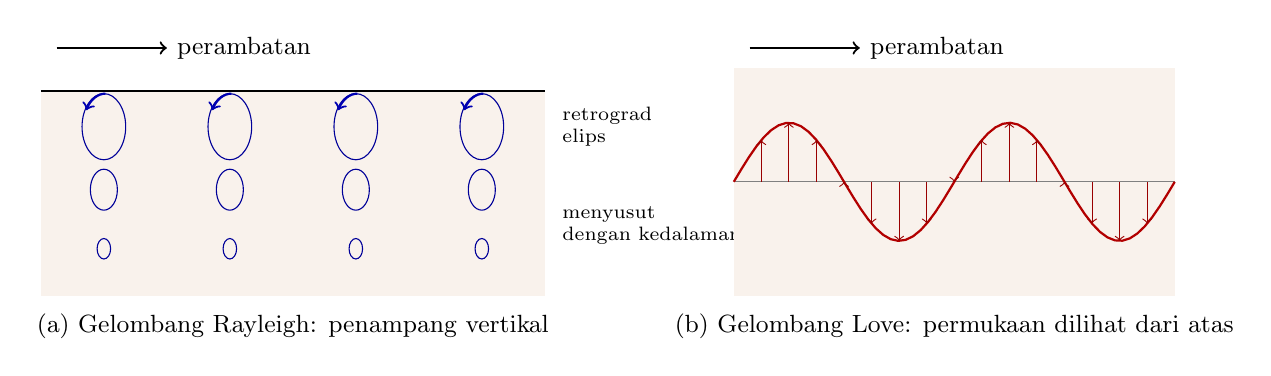
\begin{tikzpicture}[font=\small, x=1cm, y=1cm]
% Rayleigh: vertical section
\fill[brown!10] (0,0) rectangle (6.4,-2.6);
\draw[thick] (0,0) -- (6.4,0);
 \draw[->, thick] (0.2,0.55) -- (1.6,0.55) node[right] {perambatan};
\foreach \x/\s in {0.8/1, 2.4/-1, 4.0/1, 5.6/-1} {
  \foreach \z/\a in {-0.45/0.42, -1.25/0.26, -2.0/0.13} {
    \draw[blue!60!black] (\x,\z) ellipse ({0.66*\a} and {\a});
  }
}
\foreach \x in {0.8, 2.4, 4.0, 5.6} {
  \draw[->, blue!70!black, thick] (\x+0.02,-0.03) arc (90:150:{0.28} and {0.42});
}
\node[anchor=north] at (3.2,-2.7) {(a) Gelombang Rayleigh: penampang vertikal};
\node[anchor=west, font=\scriptsize, align=left] at (6.5,-0.45) {retrograd\\elips};
\node[anchor=west, font=\scriptsize, align=left] at (6.5,-1.7) {menyusut\\dengan kedalaman};
% Love: plan view of the surface
\begin{scope}[xshift=8.8cm]
\fill[brown!10] (0,0.3) rectangle (5.6,-2.6);
\draw[->, thick] (0.2,0.55) -- (1.6,0.55) node[right] {perambatan};
\draw[gray, thin] (0,-1.15) -- (5.6,-1.15);
\draw[red!70!black, thick, domain=0:5.6, samples=60] plot (\x,{-1.15+0.75*sin(\x*360/2.8)});
\foreach \x in {0.35,0.7,...,5.3} {
  \pgfmathsetmacro{\d}{0.75*sin(\x*360/2.8)}
  \draw[->, red!60!black] (\x,-1.15) -- (\x,{-1.15+\d});
}
\node[anchor=north] at (2.8,-2.7) {(b) Gelombang Love: permukaan dilihat dari atas};
\end{scope}
\end{tikzpicture}

\par\smallskip{\small Gerak partikel kedua gelombang permukaan (skematis).
(a) \omterm{def:b3:seismology-imaging:surface-waves}{Gelombang Rayleigh} menggerakkan tanah pada bidang vertikal perambatan,
sepanjang elips yang berbalik arah di bagian atas (retrograd) dekat permukaan dan
menyusut seiring kedalaman. (b) \omterm{def:b3:seismology-imaging:surface-waves}{Gelombang Love} menggerakkan tanah secara horizontal, tegak lurus
terhadap arah perambatan: panah menunjukkan pergeseran pada satu saat
sepanjang garis di permukaan.}
\label{fig:b3:seismology-imaging:particle-motion}
\end{omfigure}

\begin{theorem}[Dispersi gelombang Love dalam lapisan di atas setengah ruang]\label{thm:b3:seismology-imaging:love}
Sebuah lapisan dengan tebal $H$, modulus geser $\mu_1$ dan kecepatan S $\beta_1$ terletak di atas
setengah ruang dengan modulus geser $\mu_2$ dan kecepatan S $\beta_2 > \beta_1$. \omterm{def:b3:seismology-imaging:surface-waves}{Gelombang Love}
dengan frekuensi sudut $\omega$ dan bilangan gelombang $k$ merambat dengan
kecepatan fase $c = \omega/k$, $\beta_1 < c < \beta_2$, jika dan hanya jika
\[
  \tan\!\left(kH q_1\right) = \frac{\mu_2 q_2}{\mu_1 q_1},
  \qquad q_1 = \sqrt{\frac{c^2}{\beta_1^2} - 1},\quad
  q_2 = \sqrt{1 - \frac{c^2}{\beta_2^2}} .
\]
Mode dasar adalah akar dengan $0 < kHq_1 < \pi/2$; mode overtone memiliki
$kHq_1$ berada dalam $(n\pi, n\pi + \pi/2)$.
\end{theorem}

\begin{proof}
Ambil $x$ searah perambatan, $y$ horizontal tegak lurus terhadapnya dan $z$ ke bawah dari
permukaan bebas, dan cari pergeseran
$u_y = f(z)\,e^{i(kx - \omega t)}$, komponen lainnya nol. Setiap lapisan
memenuhi persamaan gelombang $\partial^2 u_y/\partial t^2 = \beta^2\nabla^2 u_y$, sehingga
$f'' = -k^2\left(c^2/\beta^2 - 1\right) f$. Dalam lapisan, $c > \beta_1$, dan
$f = A\cos(kq_1z) + B\sin(kq_1z)$. Dalam setengah ruang, $c < \beta_2$, dan
solusi yang tetap terbatas di kedalaman adalah $f = C\,e^{-kq_2(z - H)}$.
Traksi geser pada bidang horizontal adalah $\mu\,\partial u_y/\partial z$.
Di permukaan bebas, traksi ini bernilai nol: $f'(0) = 0$, sehingga $B = 0$. Pada $z = H$
pergeseran dan traksi kontinu:
\[
  A\cos(kq_1H) = C, \qquad -\mu_1 A\,kq_1\sin(kq_1H) = -\mu_2\,kq_2\,C .
\]
Dengan membagi persamaan kedua dengan yang pertama diperoleh hasilnya. Karena
ruas kanan positif, $kHq_1$ berada dalam seperempat periode tempat
tangennya positif; interval terkecil seperti itu menghasilkan moda dasar.
\end{proof}

Untuk periode tertentu persamaan diselesaikan untuk $c$ dengan biseksi; kecepatan grup
mengikuti dari $U = \mathrm d\omega/\mathrm dk$. Pada periode pendek
($kH$ besar) akarnya dekat $c = \beta_1$: gelombang berada di dalam lapisan. Pada
periode panjang ($kH \to 0$) harus berlaku $kHq_1 \to 0$ dengan ruas kanan
juga kecil, yang memaksa $c \to \beta_2$: gelombang mencapai jauh ke dalam
setengah ruang dan merambat dengan kecepatannya. Di antara keduanya, kecepatan fase naik
secara mantap seiring periode.

\begin{definition}[Dispersi gelombang permukaan]\label{def:b3:seismology-imaging:dispersion}
Yang disebut \emph{dispersi gelombang permukaan}\index{dispersi gelombang permukaan} adalah ketergantungan
dari kecepatan fase dan kecepatan grup \omterm{def:b3:seismology-imaging:surface-waves}{gelombang Rayleigh} atau Love terhadap periodenya. Pada
Bumi berlapis, dispersi ini muncul karena gelombang berperiode lebih panjang mencapai lebih dalam
(sekitar sepertiga panjang gelombang untuk moda dasar) dan merata-ratakan batuan yang lebih cepat;
kurva dispersi $c(T)$ dan $U(T)$ yang diukur antara gempa bumi
dan stasiun, atau antara dua stasiun, diinversi untuk memperoleh kecepatan S sebagai
fungsi kedalaman.
\end{definition}

\begin{omfigure}
\begin{tikzpicture}
\begin{axis}[omrecord, xmode=log, width=0.82\linewidth, height=0.5\linewidth,
  xmin=3, xmax=150, ymin=3.3, ymax=4.6, log basis x=10,
  xtick={3,5,10,20,50,100,150}, xticklabels={3,5,10,20,50,100,150},
  xlabel={periode $T$ (\unit{s})}, ylabel={kecepatan (\unit{km.s^{-1}})},
  legend style={at={(0.03,0.62)}, anchor=west}, legend cell align=left]
\addplot[blue!70!black, thick] table[x=period, y=c] {figdata/out/bachelor-3-love_dispersion-curve.dat};
\addlegendentry{kecepatan fase $c$}
\addplot[red!70!black, thick] table[x=period, y=U] {figdata/out/bachelor-3-love_dispersion-curve.dat};
\addlegendentry{kecepatan grup $U$}
\draw[gray, dashed] (axis cs:3,3.5) -- (axis cs:150,3.5);
\draw[gray, dashed] (axis cs:3,4.5) -- (axis cs:150,4.5);
\node[font=\scriptsize, anchor=south] at (axis cs:80,3.5) {$\beta_1 = 3.5$};
\node[font=\scriptsize, anchor=south west] at (axis cs:3.1,4.5) {$\beta_2 = 4.5$};
\addplot[only marks, mark=*, mark size=1.4pt, red!70!black] coordinates {(19.2,3.384)};
\node[font=\scriptsize, anchor=south, red!70!black] at (axis cs:19.2,3.39) {fase Airy};
\end{axis}
\end{tikzpicture}

\par\smallskip{\small \omterm{def:b3:seismology-imaging:surface-waves}{Gelombang Love} mode fundamental pada lapisan \qty{35}{km}
($\beta_1 = \qty{3.5}{km.s^{-1}}$, \qty{2.7}{g.cm^{-3}}) di atas ruang setengah
($\beta_2 = \qty{4.5}{km.s^{-1}}$, \qty{3.3}{g.cm^{-3}}), model yang disederhanakan untuk
kerak benua di atas mantel, dihitung dari
\cref{thm:b3:seismology-imaging:love}. Kecepatan fase naik dari
kecepatan gelombang S lapisan ke kecepatan ruang setengah; kecepatan grup lebih rendah dan memiliki
minimum, \qty{3.384}{km.s^{-1}} pada \qty{19.2}{s}, ketika gelombang dengan periode berdekatan
tiba bersama sebagai denyut besar yang terlambat (fase Airy).}
\label{fig:b3:seismology-imaging:love}
\end{omfigure}

Pada model ini kecepatan fase pada \qty{20}{s} adalah \qty{3.79}{km.s^{-1}} dan pada
\qty{100}{s} \qty{4.444}{km.s^{-1}}; kecepatan grup masing-masing 3.384 dan
\qty{4.333}{km.s^{-1}}. Pada seismogram yang terekam beberapa ribu kilometer
jauhnya, periode panjang tiba lebih dulu dan gelombang 20-s tiba terakhir, sehingga
kereta gelombang tertarik menjadi osilasi panjang yang perlahan memendek. Pengukuran
kecepatan grup pada banyak periode di sepanjang banyak lintasan menghasilkan peta ketebalan kerak
dan mantel paling atas, tidak bergantung pada
waktu tempuh gelombang badan.

\section{Bumi bergetar: mode normal}

Gelombang permukaan berperiode sangat panjang memiliki panjang gelombang yang sebanding dengan
jari-jari Bumi; gelombang itu menjalar mengelilingi bola dan bertemu dengan dirinya sendiri. Gelombang yang
berinterferensi konstruktif adalah gelombang berdiri seluruh bola, yaitu mode
normalnya, dan setelah gempa bumi besar, merekalah sinyal terakhir yang mereda.
Teorinya, yakni masalah nilai eigen untuk Bumi elastis yang bergravitasi sendiri, berada
di luar bab ini; deskripsinya tidak.

Mode-mode dari Bumi yang simetris bola membentuk dua keluarga. Dalam
mode \emph{toroidal}, ${}_nT_\ell$, gerakannya horizontal, yaitu puntiran
kulit-kulit bola satu terhadap yang lain, tanpa perubahan jari-jari atau volume: gelombang berdiri
dari \omterm{def:b3:seismology-imaging:surface-waves}{gelombang Love}. Pada mode \emph{sferoidal}, ${}_nS_\ell$,
gerakannya memiliki bagian radial dan horizontal, dan Bumi berubah bentuk: gelombang
berdiri dari \omterm{def:b3:seismology-imaging:surface-waves}{gelombang Rayleigh}, terkopel dengan gelombang badan dan gravitasi.
Indeks $\ell$ adalah derajat sudut, yaitu jumlah garis nodal dari
pola di permukaan; $n$ menghitung simpul gerakan terhadap jari-jari, $n = 0$
untuk mode fundamental. Mode sferoidal paling sederhana, ${}_0S_2$, meregangkan
Bumi bergantian menjadi sferoid prolat dan sferoid oblat; mode toroidal paling sederhana,
${}_0T_2$, memuntir belahan bumi utara dan belahan bumi selatan secara berlawanan
arah. Periode teramatinya adalah:
\begin{center}
\small
% ledger: seis5:modes-T, seis5:modes-S
\begin{tabular}{lcccc}
\hline
mode & ${}_0T_2$ & ${}_1T_2$ & ${}_0T_3$ & ${}_1T_3$ \\
periode (\unit{min}) & 44.01 & 12.61 & 28.43 & 11.59 \\
\hline
mode & ${}_0S_2$ & ${}_1S_2$ & ${}_0S_3$ & ${}_1S_3$ \\
periode (\unit{min}) & 53.89 & 24.51 & 35.56 & 17.68 \\
\hline
\end{tabular}
\end{center}
Setiap periode adalah rata-rata seluruh Bumi dari modulus elastisnya dan
massa jenisnya, dibobot menurut tempat mode itu bergerak: mode toroidal hanya merasakan
mantel padat dan kerak, sedangkan mode sferoidal juga merasakan inti.
Mencocokkan periode ratusan mode merupakan satu-satunya cara seismologi untuk menimbang
bagian dalam Bumi: cara ini membatasi massa jenis, bukan hanya kecepatan, dan PREM dibangun untuk
mencocokkannya bersama waktu tempuh. Rotasi dan elipsitas
Bumi memecah tiap mode berderajat $\ell$ menjadi $2\ell + 1$
frekuensi yang sedikit berbeda, analog dengan efek Zeeman.

\begin{history}[Bumi setelah gempa bumi Chili]
Gempa bumi Chili 1960 terekam oleh seismometer pendulum periode panjang
dan oleh strainmeter, instrumen yang mengukur perubahan panjang sebuah
batang atau kawat horizontal panjang yang ditambatkan pada batuan. Analisis spektral dari beberapa hari
rekaman menunjukkan puncak tajam pada periode prediksi mode paling sederhana: seluruh
Bumi telah berdering, dan prediksi teori elastis
untuk Bumi bola yang bergravitasi sendiri terpenuhi. Rekaman strainmeter
di Isabella, California, dianalisis ulang pada 1978 dengan metode yang lebih
mutakhir: ia dengan jelas menunjukkan pemecahan ${}_0T_3$, ${}_0T_4$, ${}_0S_4$
dan ${}_0S_5$ akibat rotasi dan elipsitas Bumi, serta menegaskan bahwa
hal yang sama berlaku untuk ${}_0S_2$ dan ${}_0S_3$.
% ledger: stein78:chile-modes, usgs5:chile1960
Seismologi mode normal, yang lahir dari satu gempa bumi, kini memakai jaringan
stasiun berpita sangat lebar yang merekam setiap gempa bumi besar.
\end{history}

\section{Masalah invers linear}\label{sec:b3:seismology-imaging:inverse}

Setiap metode dalam bab ini sejauh ini menghitung data dari sebuah model. Tugas
pencitraan adalah kebalikannya.

\begin{definition}[Masalah maju, masalah invers]\label{def:b3:seismology-imaging:inverse}
Misalkan model Bumi dinyatakan oleh vektor $\mathbf m$ berisi $M$ parameter
dan pengamatan oleh vektor $\mathbf d$ berisi $N$ data. Yang disebut \emph{masalah
maju}\index{masalah maju} adalah menghitung data $\mathbf d = g(\mathbf m)$
yang dihasilkan oleh model tertentu berdasarkan teori fisika. Sebaliknya, \emph{masalah
invers}\index{masalah invers} adalah menaksir model dari data yang mengandung
galat, $\mathbf d = g(\mathbf m) + \mathbf e$, dan menyatakan seberapa baik setiap bagian
model ditentukan. Masalah itu linear bila $g(\mathbf m) =
\mathsf G\mathbf m$ untuk matriks tetap $N\times M$ $\mathsf G$, disebut kernel.
\end{definition}

Mencocokkan garis lurus pada waktu tempuh adalah \omterm{def:b3:seismology-imaging:inverse}{masalah invers} linear dengan
$M = 2$ (latihan 7); tomografi waktu tempuh adalah masalah dengan ribuan
parameter. Ada tiga kasus. Jika $N > M$ dan data membatasi setiap
parameter, masalahnya \emph{terdeterminasi berlebih}: tidak ada model yang cocok dengan setiap data
persis, dan yang terbaik dicari dalam arti statistik. Jika beberapa kombinasi
parameter tidak mengubah data ($\mathsf G\mathbf m_0 = \mathbf 0$ untuk
$\mathbf m_0 \ne \mathbf 0$), masalahnya \emph{kurang terdeterminasi} pada
arah itu, dan berapa pun banyak data jenis itu tidak akan memperbaikinya. Masalah nyata
bersifat campuran: terdeterminasi berlebih di beberapa bagian model dan kurang terdeterminasi di
bagian lainnya.

\begin{theorem}[Taksiran kuadrat terkecil terbobot]\label{thm:b3:seismology-imaging:wls}
Misalkan $\mathbf d = \mathsf G\mathbf m + \mathbf e$, dengan galat $\mathbf e$
memiliki rata-rata nol dan matriks kovarians $\mathsf C_d$ (diagonal
$\sigma_i^2$ untuk galat yang saling bebas). Jika matriks
$\mathsf N = \mathsf G^{\mathsf T}\mathsf C_d^{-1}\mathsf G$ dapat dibalik, maka
model yang meminimumkan ketakcocokan
\[
  \chi^2(\mathbf m) = (\mathbf d - \mathsf G\mathbf m)^{\mathsf T}\mathsf C_d^{-1}
  (\mathbf d - \mathsf G\mathbf m)
\]
adalah \emph{taksiran kuadrat terkecil terbobot}\index{taksiran kuadrat terkecil terbobot}
\[
  \hat{\mathbf m} = \mathsf N^{-1}\mathsf G^{\mathsf T}\mathsf C_d^{-1}\mathbf d ,
\]
taksiran ini bersifat tak bias, dan matriks kovariansnya adalah
$\mathsf C_{\hat m} = \mathsf N^{-1}$.
\end{theorem}

\begin{proof}
$\chi^2$ adalah fungsi kuadrat dari $\mathbf m$ dengan gradien
$-2\mathsf G^{\mathsf T}\mathsf C_d^{-1}(\mathbf d - \mathsf G\mathbf m)$, yang
bernilai nol untuk persamaan normal $\mathsf N\mathbf m = \mathsf G^{\mathsf T}
\mathsf C_d^{-1}\mathbf d$; Hessian $2\mathsf N$ bersifat definit positif bila
$\mathsf N$ dapat dibalik (maka $\mathbf x^{\mathsf T}\mathsf N\mathbf x =
\|\mathsf C_d^{-1/2}\mathsf G\mathbf x\|^2 > 0$ untuk $\mathbf x \ne 0$), sehingga
titik stasioner itu adalah minimum. Tulis $\hat{\mathbf m} = \mathsf H\mathbf d$ dengan
$\mathsf H = \mathsf N^{-1}\mathsf G^{\mathsf T}\mathsf C_d^{-1}$. Maka
$\mathsf H\mathsf G = \mathsf I$, sehingga $\hat{\mathbf m} = \mathbf m + \mathsf H\mathbf e$
memiliki rata-rata $\mathbf m$, dan kovariansinya adalah
$\mathsf H\mathsf C_d\mathsf H^{\mathsf T} =
\mathsf N^{-1}\mathsf G^{\mathsf T}\mathsf C_d^{-1}\mathsf C_d\mathsf C_d^{-1}
\mathsf G\mathsf N^{-1} = \mathsf N^{-1}$.
\end{proof}

Pembobotan melakukan apa yang secara intuitif diharapkan: data dengan galat separuhnya
dihitung empat kali lebih berpengaruh. Matriks kovariansi memberi setiap parameter
galat bakunya $\sqrt{(\mathsf N^{-1})_{jj}}$ serta korelasi antarparameter. Jika model
benar dan galatnya berdistribusi Gaussian, $\chi^2$ minimum mengikuti hukum $\chi^2$
dengan $N - M$ derajat kebebasan: nilai yang jauh di atas $N - M$ berarti galatnya
diremehkan atau modelnya terlalu sederhana; nilai yang jauh di bawahnya berarti galatnya
dilebih-lebihkan.

Jika $\mathsf N$ singular atau hampir singular, taksiran tidak ada atau
didominasi oleh derau yang diperbesar sepanjang arah yang kurang terkendala. Obat
standar adalah mencari model yang cocok dengan data secara wajar dan tidak
berukuran berlebihan.

\begin{definition}[Kuadrat terkecil teredam, kurva kompromi]\label{def:b3:seismology-imaging:damped}
Untuk parameter redaman $\varepsilon > 0$, taksiran \emph{kuadrat terkecil
teredam}\index{kuadrat terkecil teredam} adalah model yang meminimalkan
\[
  \Phi_\varepsilon(\mathbf m) = \chi^2(\mathbf m) + \varepsilon^2\|\mathbf m\|^2 ,
  \qquad
  \mathbf m_\varepsilon = \left(\mathsf N + \varepsilon^2\mathsf I\right)^{-1}
  \mathsf G^{\mathsf T}\mathsf C_d^{-1}\mathbf d .
\]
Yang disebut \emph{kurva kompromi}\index{kurva kompromi} adalah kurva yang ditelusuri ketika
$\varepsilon$ bervariasi, oleh pasangan (ukuran model $\|\mathbf m_\varepsilon\|$,
ketakcocokan $\chi^2(\mathbf m_\varepsilon)$): redaman kecil mencocokkan data dengan erat
dengan model yang besar dan kasar; redaman besar memberikan model yang kecil dan kecocokan yang buruk.
\end{definition}

Rumus ini diperoleh seperti pada \cref{thm:b3:seismology-imaging:wls}: gradien
dari $\Phi_\varepsilon$ adalah $-2\mathsf G^{\mathsf T}\mathsf C_d^{-1}(\mathbf d -
\mathsf G\mathbf m) + 2\varepsilon^2\mathbf m$, dan $\mathsf N + \varepsilon^2
\mathsf I$ selalu dapat dibalik, sebab nilai eigennya adalah nilai eigen
$\mathsf N$ (semuanya $\ge 0$) yang masing-masing ditambah $\varepsilon^2$. Redaman biasanya
dipilih di dekat lutut \omterm{def:b3:seismology-imaging:damped}{kurva kompromi}, atau sedemikian rupa sehingga $\chi^2$ kira-kira
sama dengan jumlah data, yaitu ketakcocokan yang diharapkan dari galat saja. Harganya ialah bahwa
taksiran itu tidak lagi tak bias.

\begin{definition}[Matriks resolusi model]\label{def:b3:seismology-imaging:resolution}
Untuk taksiran linear $\mathbf m_\varepsilon = \mathsf H_\varepsilon \mathbf d$
untuk model $\mathbf m$ dari data $\mathbf d = \mathsf G\mathbf m + \mathbf e$,
yang disebut \emph{matriks resolusi model}\index{matriks resolusi model} adalah
$\mathsf R = \mathsf H_\varepsilon\mathsf G$, sehingga
\[
  \mathbf m_\varepsilon = \mathsf R\,\mathbf m + \mathsf H_\varepsilon\mathbf e .
\]
Untuk \omterm{def:b3:seismology-imaging:damped}{kuadrat terkecil teredam}, $\mathsf R = (\mathsf N + \varepsilon^2\mathsf I)^{-1}
\mathsf N$. Baris $j$ dari $\mathsf R$ menunjukkan bagaimana taksiran parameter $j$
merata-ratakan parameter sebenarnya; $\mathsf R = \mathsf I$ berarti resolusi sempurna.
\end{definition}

Jika $\mathsf N$ memiliki vektor eigen ortonormal $\mathbf u_k$ dan nilai eigen
$\lambda_k$, maka $\mathsf R = \sum_k \frac{\lambda_k}{\lambda_k + \varepsilon^2}
\mathbf u_k\mathbf u_k^{\mathsf T}$: arah yang dikendalikan data dengan baik
($\lambda_k \gg \varepsilon^2$) tetap hampir tidak berubah, sedangkan arah yang
dikendalikan data dengan buruk ditekan. Jejak $\mathsf R$ menghitung parameter yang
secara efektif diresolusi data, dan kovariansi taksiran,
$\mathsf H_\varepsilon\mathsf C_d\mathsf H_\varepsilon^{\mathsf T}$, menyusut seiring
dengan menurunnya resolusi: redaman menukar resolusi dengan kestabilan.

\begin{omfigure}
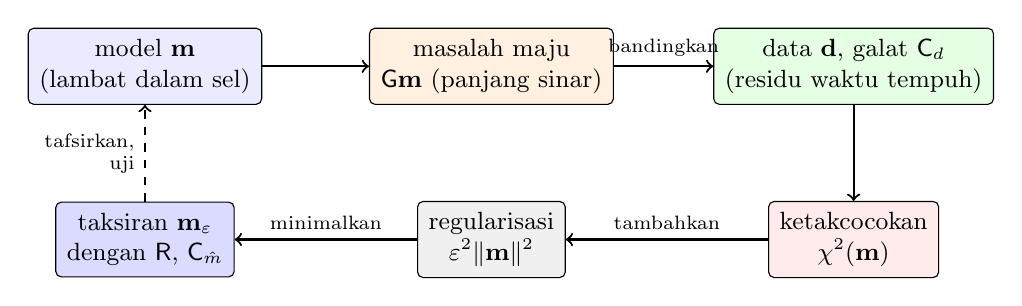
\begin{tikzpicture}[font=\small, node distance=0.5cm,
  box/.style={draw, rounded corners=2pt, fill=#1, minimum height=0.9cm, align=center, inner sep=4pt},
  box/.default=gray!8]
\node[box=blue!8] (m) at (0,0) {model $\mathbf m$\\(lambat dalam sel)};
\node[box=orange!12] (g) at (4.4,0) {masalah maju\\$\mathsf G\mathbf m$ (panjang sinar)};
\node[box=green!10] (d) at (9.0,0) {data $\mathbf d$, galat $\mathsf C_d$\\(residu waktu tempuh)};
\node[box=red!8] (mis) at (9.0,-2.2) {ketakcocokan\\$\chi^2(\mathbf m)$};
\node[box=gray!12] (reg) at (4.4,-2.2) {regularisasi\\$\varepsilon^2\|\mathbf m\|^2$};
\node[box=blue!14] (est) at (0,-2.2) {taksiran $\mathbf m_\varepsilon$\\dengan $\mathsf R$, $\mathsf C_{\hat m}$};
\draw[->, thick] (m) -- (g);
\draw[->, thick] (g) -- node[above, font=\scriptsize] {bandingkan} (d);
\draw[->, thick] (d) -- (mis);
\draw[->, thick] (mis) -- node[above, font=\scriptsize] {tambahkan} (reg);
\draw[->, thick] (reg) -- node[above, font=\scriptsize] {minimalkan} (est);
\draw[->, thick, dashed] (est) -- node[left, font=\scriptsize, align=right] {tafsirkan,\\uji} (m);
\end{tikzpicture}

\par\smallskip{\small \omterm{def:b3:seismology-imaging:inverse}{Masalah invers} linear sebagai lingkaran (skematik). \omterm{def:b3:seismology-imaging:inverse}{Masalah
maju} memprediksi data dari sebuah model; ketakcocokan, yang diberi bobot menurut galat data,
mengukur ketidaksesuaian; suku regularisasi menjaga agar model
tetap kecil; meminimalkan jumlahnya menghasilkan taksiran, yang hanya dapat ditafsirkan
bersama matriks resolusi dan kovariansinya.}
\label{fig:b3:seismology-imaging:inverse-loop}
\end{omfigure}

\section{Tomografi seismik}\label{sec:b3:seismology-imaging:tomography}

\begin{definition}[Tomografi seismik, residu waktu tempuh]\label{def:b3:seismology-imaging:tomography}
Yang disebut \emph{residu waktu tempuh}\index{residu waktu tempuh} dari sebuah fase yang tiba adalah
waktu tempuh terukur dikurangi waktu yang diprediksi oleh model acuan,
$\delta t = T_{\text{obs}} - T_{\text{ref}}$, setelah dikoreksi terhadap lokasi
sumber dan waktu asal, elevasi stasiun, serta
elipsitas Bumi. Yang disebut \emph{tomografi seismik}\index{tomografi seismik} adalah
taksiran simpangan tiga dimensi kecepatan seismik dari sebuah
model acuan, $\delta v(\mathbf x)$, dari sekumpulan besar residu (atau
bentuk gelombang), dengan menyelesaikan \omterm{def:b3:seismology-imaging:inverse}{masalah invers}.
\end{definition}

Tulis $s = 1/v$ untuk kelambatan. Waktu tempuh sepanjang sinar $\Gamma$ adalah
$T = \int_\Gamma s\,\mathrm dl$; namun sinarnya sendiri bergantung pada kecepatan,
yang tampaknya membuat masalahnya tak-linear. Jawaban orde pertama adalah bahwa hal itu
tidak berpengaruh.

\begin{proposition}[Residu waktu tempuh terlinearisasi]\label{prop:b3:seismology-imaging:linear}
Jika kelambatan model acuan $s_0$ diganggu menjadi $s_0 + \delta s$,
waktu tempuh antara dua titik tetap berubah, hingga orde pertama dalam
$\delta s$, sebesar
\[
  \delta t = \int_{\Gamma_0}\delta s\,\mathrm dl ,
\]
dengan integral dihitung sepanjang sinar $\Gamma_0$ dari model acuan; anomali
kecepatan relatif adalah $\delta v/v_0 = -\delta s/s_0$ pada orde yang sama.
\end{proposition}

\begin{proof}
Menurut prinsip Fermat, sinar $\Gamma_0$ membuat waktu tempuh
$\int s_0\,\mathrm dl$ stasioner terhadap lintasan tetangga: menggeser lintasan dengan
sejumlah kecil $\epsilon$ hanya mengubah waktu sebesar suku berorde $\epsilon^2$.
Sinar baru $\Gamma$ berbeda dari $\Gamma_0$ sebesar orde $\delta s$;
sehingga $\int_\Gamma(s_0 + \delta s)\,\mathrm dl = \int_{\Gamma_0}s_0\,\mathrm dl +
O(\delta s^2) + \int_{\Gamma_0}\delta s\,\mathrm dl + O(\delta s^2)$. Akhirnya
$\delta(1/s) = -\delta s/s_0^2$, sehingga $\delta v/v_0 = -\delta s/s_0$.
\end{proof}

Bagi daerah itu menjadi $M$ sel dengan gangguan kelambatan seragam $\delta s_j$.
Residu sinar $i$ menjadi $\delta t_i = \sum_j L_{ij}\,\delta s_j$, dengan
$L_{ij}$ adalah panjang sinar acuan $i$ dalam sel $j$: sebuah \omterm{def:b3:seismology-imaging:inverse}{masalah invers} linear
dengan kernel berupa matriks panjang sinar, yang hampir semua entrinya
bernilai nol. Residunya kecil: di mantel dengan
\qty{8}{km.s^{-1}}, sebuah daerah selebar \qty{200}{km} yang \qty{3}{\percent}
lebih cepat, sehingga sinar vertikal tiba sekitar \qty{0.7}{s} lebih awal (latihan 9).

\begin{method}[Tomografi waktu tempuh]\label{met:b3:seismology-imaging:tomo}
\begin{enumerate}
  \item Pilih waktu tiba satu fase (misalnya P) di semua stasiun, untuk
        gempa bumi yang lokasinya diketahui dengan baik; hitung residunya
        terhadap \omterm{def:b3:seismology-imaging:tables}{tabel waktu tempuh}, dikoreksi terhadap elipsitas dan
        elevasi stasiun.
  \item Telusuri sinar acuan dan bagi daerah menjadi sel (atau
        uraikan $\delta s$ dalam fungsi halus); isi matriks panjang sinar.
  \item Berikan setiap residu galatnya, dari presisi pembacaan waktu tiba, lalu selesaikan
        masalah \omterm{def:b3:seismology-imaging:damped}{kuadrat terkecil teredam} untuk sejumlah nilai redaman; gambarkan
        \omterm{def:b3:seismology-imaging:damped}{kurva kompromi}, dan pilih redaman di dekat titik lengkungnya.
  \item Uji resolusinya: hitung residu yang dihasilkan model sintetik yang diketahui
        melalui sinar yang sama, tambahkan derau, lalu lakukan inversi dengan
        redaman yang sama, lalu bandingkan.
  \item Tafsirkan hanya anomali yang menurut uji dapat dipulihkan
        oleh sinar, dengan amplitudonya dipahami sebagai batas bawah.
\end{enumerate}
\end{method}

\begin{definition}[Uji papan catur]\label{def:b3:seismology-imaging:checkerboard}
Yang disebut \emph{uji papan catur}\index{uji papan catur} adalah uji resolusi,
dengan model sintetik berupa pola teratur sel-sel cepat dan lambat yang bergantian:
residu sintetik yang dihitung melalui geometri sinar sebenarnya, dengan derau
berukuran sama dengan galat sebenarnya, diinversi dengan parametrisasi dan
redaman yang sama. Bila pola itu dapat dipulihkan, struktur seukuran itu dapat
diresolusi; bila pola itu kabur atau hilang, struktur itu tidak.
\end{definition}

Gambar-gambar di bawah menjalankan uji ini pada penampang model selebar \qty{800}{km} dan
\qty{400}{km} dalamnya, dibagi menjadi 128 sel masing-masing \qty{50}{km}. Dua puluh sumber terletak
di sepanjang dasarnya dan tiga puluh dua stasiun di sepanjang puncaknya, dan hanya sinar dalam
\ang{45} dari vertikal yang dipakai: 480 sinar yang semuanya merambat curam ke atas,
geometri sinar dari gempa bumi jauh yang naik di bawah jaringan.
Model sintetik memiliki blok berukuran $2\times2$ sel, \qty{3}{\percent} lebih cepat atau lebih lambat
di sekitar \qty{8}{km.s^{-1}}; residunya membawa derau Gauss sebesar
\qty{0.05}{s}.
% figdata: tomo_checkerboard.py (invented geometry; no real data)

\begin{omfigure}
\begin{tikzpicture}
\begin{groupplot}[group style={group size=2 by 2, horizontal sep=0.9cm, vertical sep=1.25cm},
  width=0.46\linewidth, height=0.3\linewidth, xmin=0, xmax=800, ymin=0, ymax=400,
  axis on top, enlargelimits=false, tick label style={font=\scriptsize},
  title style={font=\small, yshift=-1ex},
  colormap={tomo}{rgb255(0cm)=(178,24,43); rgb255(1cm)=(244,165,130); rgb255(2cm)=(247,247,247); rgb255(3cm)=(146,197,222); rgb255(4cm)=(33,102,172)},
  point meta min=-4, point meta max=4]
\nextgroupplot[title={(a) model sintetik}, ylabel={\scriptsize ketinggian (km)}]
\addplot[matrix plot*, mesh/cols=16, point meta=explicit] table[x=x, y=y, meta=dv] {figdata/out/bachelor-3-tomo_checkerboard-true.dat};
\nextgroupplot[title={(b) contoh 480 sinar}, colormap/blackwhite]
\addplot[gray!70!black, thin, unbounded coords=jump] table[x=x, y=y] {figdata/out/bachelor-3-tomo_checkerboard-rays.dat};
\addplot[only marks, mark=triangle*, mark size=1.6pt, black, clip=false] table[x=x, y=y] {figdata/out/bachelor-3-tomo_checkerboard-receivers.dat};
\addplot[only marks, mark=star, mark size=1.8pt, red!70!black, clip=false] table[x=x, y=y] {figdata/out/bachelor-3-tomo_checkerboard-sources.dat};
\nextgroupplot[title={(c) hasil pemulihan, $\varepsilon = \qty{3}{km}$}, ylabel={\scriptsize ketinggian (km)}, xlabel={\scriptsize jarak (km)}]
\addplot[matrix plot*, mesh/cols=16, point meta=explicit] table[x=x, y=y, meta=dv] {figdata/out/bachelor-3-tomo_checkerboard-rec-low.dat};
\nextgroupplot[title={(d) hasil pemulihan, $\varepsilon = \qty{60}{km}$}, xlabel={\scriptsize jarak (km)},
  colorbar right, colorbar style={width=0.2cm, ytick={-4,-2,0,2,4}, ylabel={\scriptsize $\delta v/v$ (\%)}, tick label style={font=\scriptsize}}]
\addplot[matrix plot*, mesh/cols=16, point meta=explicit] table[x=x, y=y, meta=dv] {figdata/out/bachelor-3-tomo_checkerboard-rec-high.dat};
\end{groupplot}
\end{tikzpicture}

\par\smallskip{\small \omterm{def:b3:seismology-imaging:checkerboard}{Uji papan catur} (geometri rekaan). (a) Model
sintetik: blok selebar \qty{100}{km}, \qty{3}{\percent} lebih cepat (biru) atau
lebih lambat (merah). (b) 20 sumber (bintang), 32
stasiun (segitiga) dan beberapa sinar, semuanya dalam \ang{45} dari vertikal. (c) Dengan
redaman ringan, blok-blok ditemukan, tetapi berderau, dengan anomali hingga sekitar
\qty{8}{\percent} di tempat sedikit sinar berpotongan (warna jenuh pada
\qty{4}{\percent}). (d) Dengan redaman kuat, polanya bersih, tetapi
amplitudonya berkurang, terutama di sepanjang tepi sisi, tempat sedikit sinar berpotongan
dan semuanya pada sudut serupa.}
\label{fig:b3:seismology-imaging:checkerboard}
\end{omfigure}

\begin{omfigure}
\begin{tikzpicture}
\begin{axis}[omrecord, width=0.62\linewidth, height=0.42\linewidth,
  xlabel={norma model $\|\delta v/v\|$ (\unit{\percent})},
  ylabel={ketakcocokan $\|\mathsf G\mathbf m - \mathbf d\|$ (\unit{s})}, xmin=0, xmax=42, ymin=0, ymax=12]
\addplot[blue!70!black, thick] table[x=norm, y=misfit] {figdata/out/bachelor-3-tomo_checkerboard-tradeoff.dat};
\addplot[only marks, mark=*, mark size=1.8pt, red!70!black] coordinates {(38.84,0.862) (29.42,1.159)};
\node[font=\scriptsize, anchor=south, red!70!black] at (axis cs:38.84,1.3) {$\varepsilon = 3$};
\node[font=\scriptsize, anchor=east, red!70!black] at (axis cs:28.6,0.55) {$\varepsilon = 60$};
\draw[gray, dashed] (axis cs:0,1.095) -- (axis cs:42,1.095);
\node[font=\scriptsize, anchor=south west] at (axis cs:1,1.15) {diharapkan dari derau};
\draw[green!45!black, densely dotted] (axis cs:33.94,0) -- (axis cs:33.94,12);
\node[font=\scriptsize, anchor=north west, green!45!black] at (axis cs:34.2,11.8) {model sebenarnya};
\node[font=\scriptsize, anchor=west] at (axis cs:14,10.5) {redaman kuat};
\node[font=\scriptsize, anchor=east] at (axis cs:41,3.2) {redaman ringan};
\end{axis}
\end{tikzpicture}

\par\smallskip{\small \omterm{def:b3:seismology-imaging:damped}{Kurva kompromi} \omterm{def:b3:seismology-imaging:checkerboard}{uji papan catur} untuk redaman
nilai $\varepsilon$ dari 0.1 sampai \qty{1000}{km} (kernel dalam kilometer,
dengan galat yang sama). Di sepanjang bagian datar, redaman yang lebih besar hampir tidak mengorbankan kecocokan: model
menyusut karena ikut membuang derau. Titik lutut berada di tempat ketakcocokan naik melewati
tingkat yang diharapkan dari derau saja, $\sigma\sqrt{480} = \qty{1.095}{s}$; dua
model teredam pada gambar sebelumnya terletak di kedua sisinya, dan norma
papan catur sebenarnya, \qty{33.9}{\percent}, berada di antaranya. Di luar
titik lutut, redaman menghilangkan struktur yang dibutuhkan data.}
\label{fig:b3:seismology-imaging:tradeoff}
\end{omfigure}

Uji ini menggambarkan tiga batas setiap citra tomografi. Resolusi
ditentukan oleh sinar: jika semua sinar sejajar, anomali tersebar sepanjang
sinar-sinar itu, dan sel yang dilintasi sedikit sinar hampir tidak terkendali. Redaman menurunkan
amplitudo: anomali yang diperoleh merupakan batas bawah.
Citra juga bergantung pada model acuan dan parametrisasi: hanya
simpangan dari acuan yang dipetakan, dan tidak ada yang lebih kecil dari sel.
Dengan kehati-hatian ini, citra gelombang P dan S global memperlihatkan lempengan
dari volume Tahun 1 (pada bab subduksinya) sebagai daerah cepat berbentuk tabular yang turun
dari palung, sebagian mendatar di atas diskontinuitas 670-km, sebagian lain
menghunjam ke mantel bawah; serta daerah lambat yang luas di bawah Pasifik dan
Afrika di atas inti, dengan saluran lambat yang lebih sempit di bawah beberapa titik panas, yang
merupakan kandidat untuk plume mantel dalam volume yang sama.

\begin{inthefield}[Stasiun pita lebar dan pemasangan di dasar laut]
\begin{minipage}[t]{0.55\linewidth}\vspace{0pt}
Stasiun pita lebar permanen adalah tempat yang tenang: seismometer berdiri di atas
pilar beton yang dibaut ke batuan dasar di dalam ruang bawah tanah atau terowongan pendek, di bawah
perisai termal, karena hembusan angin atau perubahan beberapa perseratus derajat
memiringkan instrumen lebih dari gempa bumi yang jauh. Tiga komponennya,
vertikal, utara, dan timur, didigitasi terus-menerus dan dikirim ke pusat data
dengan cap waktu satelit. Untuk mencitrakan wilayah di bawah samudra, tim survei
sebagai gantinya menurunkan seismometer dasar samudra dari kapal: masing-masing tenggelam dengan jangkar,
merekam selama setahun di dasar laut, lalu naik ke permukaan saat kapal
kembali dan mengirim sinyal akustik untuk melepaskannya. Awak lalu membaca
penyimpangan jamnya, mengoreksi rekaman, dan menambahkan ribuan kedatangan gelombang ke
tomografi.
\end{minipage}\hfill
\begin{minipage}[t]{0.42\linewidth}\vspace{0pt}
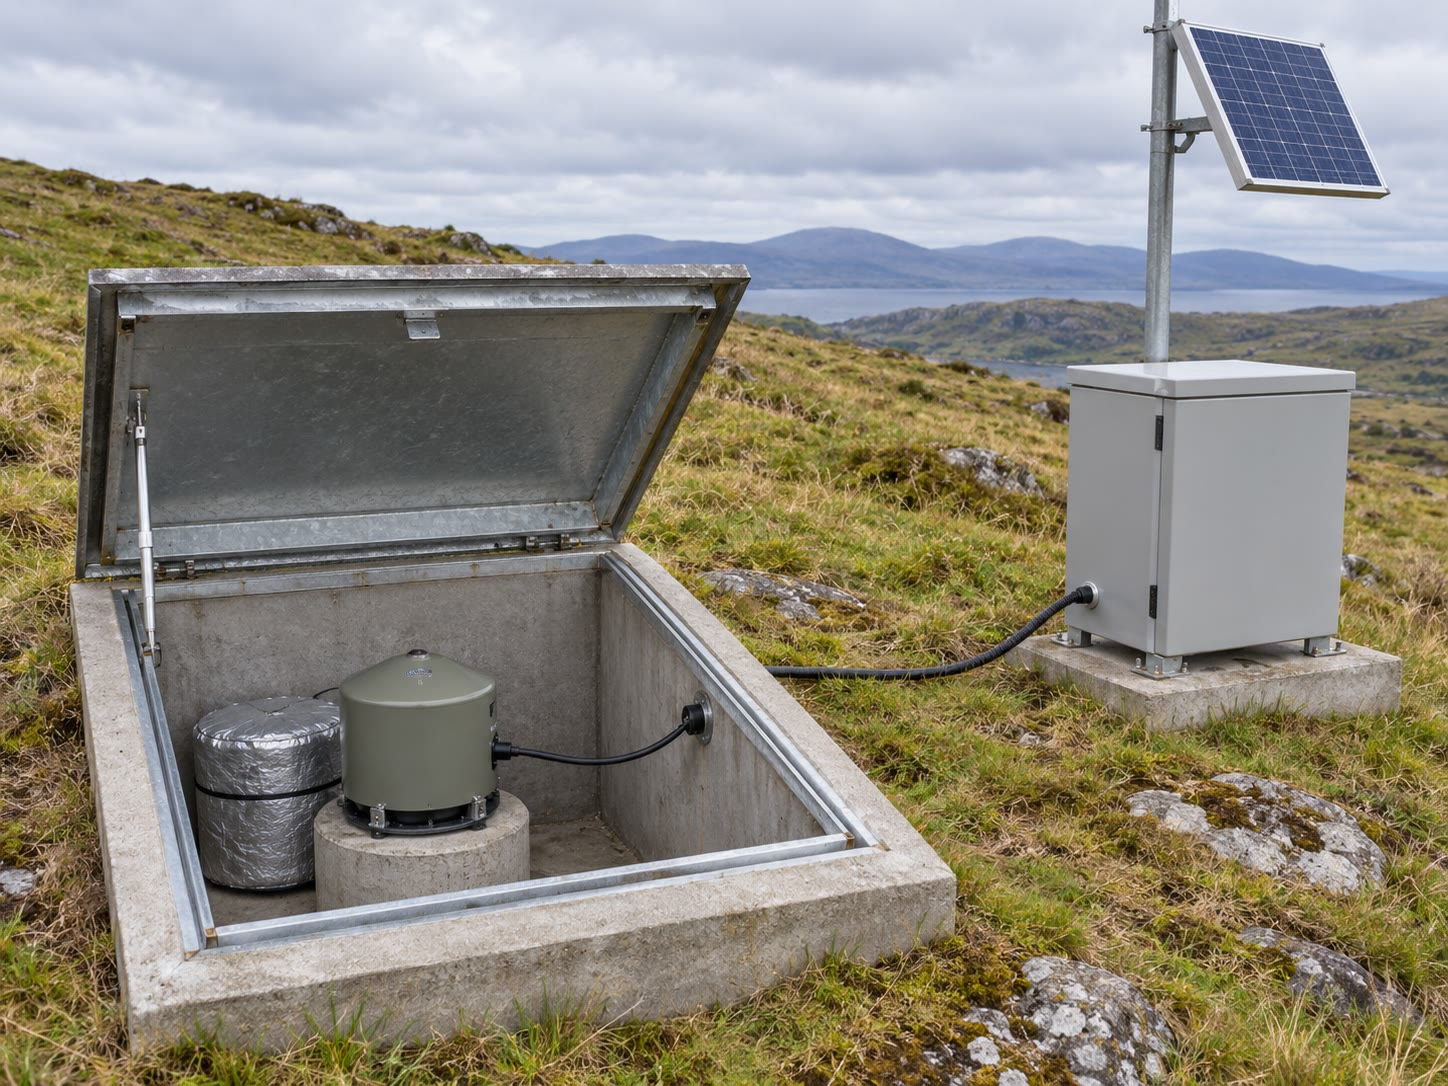
\includegraphics[width=\linewidth]{images/book5/ai/b3-seismic-vault.jpg}

{\scriptsize Seismometer pita lebar di atas pilarnya dalam ruang stasiun
(ilustrasi buatan AI).}
\end{minipage}
\end{inthefield}

\section{Latihan}

\begin{exercise}[$\star$]\label{exo:b3:seismology-imaging:1}
Sinar P meninggalkan permukaan ($R = \qty{6371}{km}$, $v_0 = \qty{5.80}{km.s^{-1}}$)
dengan \omterm{def:b3:seismology-imaging:ray-parameter}{parameter sinar} $p = \qty{500}{s.rad^{-1}}$. (a) Hitung sudut
keluarnya. (b) PREM memberikan kelajuan P sebesar \qty{11.066}{km.s^{-1}} pada kedalaman \qty{771}{km}
dan \qty{11.245}{km.s^{-1}} pada \qty{871}{km}. Hitung $r/v$ pada kedua kedalaman dan
tentukan kedalaman \omterm{def:b3:seismology-imaging:ray-parameter}{titik balik} sinar dengan interpolasi linear.
% ledger: ak135:crust, data:prem
\end{exercise}

\begin{exercise}[$\star$]\label{exo:b3:seismology-imaging:2}
Waktu P yang dihitung melalui PREM di bab ini adalah \qty{369.6}{s} pada \ang{30}
dan \qty{455.5}{s} pada \ang{40}. (a) Perkirakan kemiringan kurva waktu tempuh
antara keduanya, dalam \unit{s} per derajat dan dalam \unit{s.rad^{-1}}. (b) Turunkan
kelajuan semu front gelombang sepanjang permukaan, dalam
\unit{km.s^{-1}}. (c) Berapa kelajuan P di \omterm{def:b3:seismology-imaging:ray-parameter}{titik balik} sinar
yang tiba pada \ang{35}, jika sinar itu berbalik pada jari-jari \qty{5450}{km}?
\end{exercise}

\begin{exercise}[$\star$]\label{exo:b3:seismology-imaging:3}
Pada model \omterm{def:b3:seismology-imaging:surface-waves}{gelombang Love} di bab ini, lapisan memiliki $\beta_1 =
\qty{3.5}{km.s^{-1}}$, $\rho_1 = \qty{2700}{kg.m^{-3}}$ dan ruang setengah
$\beta_2 = \qty{4.5}{km.s^{-1}}$, $\rho_2 = \qty{3300}{kg.m^{-3}}$.
(a) Hitung kedua modulus geser. (b) Pada \qty{20}{s} kelajuan fasa adalah
\qty{3.79}{km.s^{-1}}: hitung panjang gelombangnya dan bandingkan dengan lapisan
setebal \qty{35}{km}. (c) Dengan kelajuan grup \qty{3.384}{km.s^{-1}} pada
\qty{20}{s} dan \qty{4.333}{km.s^{-1}} pada \qty{100}{s}, berapa menit
gelombang 20-s tiba setelah gelombang 100-s di stasiun yang berjarak \qty{4000}{km}?
\end{exercise}

\begin{exercise}[$\star$]\label{exo:b3:seismology-imaging:4}
Periode teramati ${}_0S_2$ dan ${}_0T_2$ adalah \qty{53.89}{min} dan
\qty{44.01}{min}. (a) Hitung frekuensinya dalam \unit{mHz}. (b) Berapa
osilasi masing-masing yang dilakukan Bumi dalam sehari? (c) Dua puncak spektral
dapat dipisahkan hanya jika rekaman berlangsung setidaknya sama dengan kebalikan
selisih frekuensinya. Berapa lama rekaman harus berlangsung untuk memisahkan kedua moda ini?
% ledger: seis5:modes-S, seis5:modes-T
\end{exercise}

\begin{exercise}[$\star\star$]\label{exo:b3:seismology-imaging:5}
Dalam bola berjari-jari $R$ dan kelajuan seragam $v$, sinar berupa tali busur lurus.
(a) Tunjukkan bahwa sinar yang mencapai $\Delta$ memiliki waktu tempuh
$T = 2R\sin(\Delta/2)/v$. (b) Dengan $R = \qty{6371}{km}$ dan
$v = \qty{10.0}{km.s^{-1}}$, hitung $T$ pada \ang{30} dan \ang{90}, dan bandingkan
dengan waktu PREM, \qty{369.6}{s} dan \qty{779.7}{s}. (c) Jelaskan mengapa
bola seragam terlalu cepat pada \ang{30} dan terlalu lambat pada \ang{90}.
\end{exercise}

\begin{exercise}[$\star\star$]\label{exo:b3:seismology-imaging:6}
Pada benda padat Poisson ($\lambda = \mu$, sehingga $\alpha^2 = 3\beta^2$) kelajuan \omterm{def:b3:seismology-imaging:surface-waves}{gelombang Rayleigh}
$c$ memenuhi, dengan $\xi = c^2/\beta^2$,
$(2 - \xi)^2 = 4\sqrt{1 - \xi/3}\,\sqrt{1 - \xi}$. (a) Kuadratkan lalu tunjukkan
bahwa akar-akarnya memenuhi $(\xi - 4)(3\xi^2 - 12\xi + 8) = 0$. (b) Tunjukkan bahwa
satu-satunya akar dengan $0 < \xi < 1$ adalah $\xi = 2 - 2/\sqrt3$, dan hitung $c/\beta$.
(c) Pada kerak atas ak135, $\beta = \qty{3.46}{km.s^{-1}}$: hitung
kelajuan Rayleigh dan keterlambatan \omterm{def:b3:seismology-imaging:surface-waves}{gelombang Rayleigh} di belakang gelombang S pada
\qty{1000}{km}.
% ledger: ak135:crust
\end{exercise}

\begin{exercise}[$\star\star$]\label{exo:b3:seismology-imaging:7}
Kedatangan gelombang kepala di empat stasiun pada garis refraksi, pada 50, 100, 150 dan
\qty{200}{km} dari titik tembak, berturut-turut 9.0, 15.3, 21.5 dan \qty{27.9}{s}, dengan
galat 0.1, 0.1, 0.2 dan \qty{0.2}{s}. Cocokkan $T = a + bx$ dengan kuadrat terkecil
terbobot: tulis $\mathsf G$ dan $\mathsf C_d$, bentuk persamaan normalnya, dan
berikan $a$, $b$, galat baku masing-masing, kelajuan $1/b$ beserta galatnya, dan
$\chi^2$ minimum. Apakah kecocokan ini dapat diterima?
\end{exercise}

\begin{exercise}[$\star\star$]\label{exo:b3:seismology-imaging:8}
Satu sinar melintasi dua sel, dengan panjang \qty{30}{km} dan \qty{40}{km}, serta
memiliki residu \qty{0.50}{s}. (a) Mengapa $\mathsf N = \mathsf G^{\mathsf T}
\mathsf G$ singular? (b) Di antara model yang mencocokkan residu secara tepat, yang
bernorma terkecil adalah $\mathbf m = \mathsf G^{\mathsf T}(\mathsf G\mathsf
G^{\mathsf T})^{-1}\mathbf d$: hitung. (c) Hitung matriks
$\mathsf R = \mathsf G^{\mathsf T}(\mathsf G\mathsf G^{\mathsf T})^{-1}\mathsf G$
dan jejaknya. (d) Jika anomali sebenarnya \qty{0.01}{s.km^{-1}} di sel pertama
saja, apa yang diperoleh kembali?
\end{exercise}

\begin{exercise}[$\star\star$]\label{exo:b3:seismology-imaging:9}
Suatu daerah lempengan di mantel \qty{3}{\percent} lebih cepat daripada sekitarnya,
dengan $v = \qty{9.0}{km.s^{-1}}$. (a) Hitung residu sinar yang melintasi
\qty{200}{km} secara vertikal, menurut \cref{prop:b3:seismology-imaging:linear},
dan secara eksak. (b) Hal yang sama untuk sinar yang melintasi ketebalan \qty{100}{km} darinya pada
\ang{40} dari garis normal terhadap lempengan. (c) Berapakah galat relatif dari
linearisasi?
\end{exercise}

\begin{exercise}[$\star\star\star$]\label{exo:b3:seismology-imaging:10}
Pada \cref{thm:b3:seismology-imaging:love}, nada atas orde $n$ hanya ada
pada periode yang cukup pendek. (a) Tunjukkan bahwa pada batas potongnya kecepatan fasenya
$\beta_2$ dan $kHq_1 = n\pi$. (b) Turunkan frekuensi sudut potong
$\omega_n = n\pi\beta_1\beta_2/\bigl(H\sqrt{\beta_2^2 - \beta_1^2}\bigr)$.
(c) Hitung periode potong nada atas pertama untuk model bab ini
($H = \qty{35}{km}$, $\beta_1 = 3.5$, $\beta_2 = \qty{4.5}{km.s^{-1}}$).
(d) Tunjukkan bahwa moda dasar tidak memiliki batas potong, dan bahwa kecepatan fasenya
cenderung ke $\beta_1$ pada periode pendek.
\end{exercise}

\begin{exercise}[$\star\star\star$]\label{exo:b3:seismology-imaging:11}
Ambil sinar pada latihan 8, dengan galat data satuan. (a) Tunjukkan bahwa, untuk
$\varepsilon > 0$, $(\mathsf G^{\mathsf T}\mathsf G + \varepsilon^2\mathsf
I)^{-1}\mathsf G^{\mathsf T} = \mathsf G^{\mathsf T}(\mathsf G\mathsf
G^{\mathsf T} + \varepsilon^2\mathsf I)^{-1}$. (b) Turunkan
matriks resolusi teredam $\mathsf R_\varepsilon = \mathsf G^{\mathsf T}\mathsf G/(\|\mathbf g\|^2 +
\varepsilon^2)$, dengan $\mathbf g = (30, 40)$, dan jejaknya. (c) Hitung
jejak dan residu data untuk $\varepsilon^2 = 0$, 2500 dan \num{10000}
(dalam \unit{km^2}). Jelaskan kompromi tersebut.
\end{exercise}

\begin{exercise}[$\star\star\star$]\label{exo:b3:seismology-imaging:12}
Pada bola homogen latihan 5: (a) tunjukkan dengan
\cref{thm:b3:seismology-imaging:benndorf} bahwa $p(\Delta) = (R/v)\cos(\Delta/2)$,
dan periksa terhadap definisi $p$ (sudut keberangkatan suatu tali busur).
(b) Tunjukkan bahwa sinar yang mencapai $\Delta_1$ memiliki \omterm{def:b3:seismology-imaging:ray-parameter}{titik balik} di $r_1 = R\cos(\Delta_1/2)$.
(c) Dengan menerima bahwa $\int_0^{\Delta_1}\operatorname{arccosh}\bigl(\cos(\Delta/2)
/\cos(\Delta_1/2)\bigr)\,\mathrm d\Delta = \pi\ln\bigl(1/\cos(\Delta_1/2)\bigr)$,
tunjukkan bahwa rumus \omterm{prop:b3:seismology-imaging:herglotz}{inversi Herglotz--Wiechert} menghasilkan $r_1$ dan kelajuan $v$.
\end{exercise}

\section{Soal: Lempengan di bawah Stasiun K}

\begin{problem}[{Soal akhir pekan --- sinar, gelombang Love dan tomografi kecil
di bawah stasiun rekaan}]
\label{pb:b3:seismology-imaging:1}
% values: calc/ch01.py (invented station and models; Love-wave model as in the chapter)
Stasiun K berdiri di atas benua, di atas zona subduksi. Soal ini memakai rekamannya
dengan tiga cara: sinar di dalam kerak, dispersi \omterm{def:b3:seismology-imaging:surface-waves}{gelombang Love} yang melintasinya,
dan tomografi kecil mantel di bawahnya.

\medskip
\noindent\textbf{Bagian I --- Sinar dalam gradien.} Pada jarak yang cukup pendek untuk
mengabaikan kelengkungan Bumi, kelajuan gelombang P di bawah K naik secara linear terhadap kedalaman,
$v(z) = v_0 + gz$, dengan $v_0 = \qty{5.0}{km.s^{-1}}$ dan
$g = \qty{0.05}{s^{-1}}$ ($z$ dalam km).
\begin{enumerate}
  \item Pada lapisan datar, hukum Snell menjaga $p = \sin i/v$ tetap. Sebuah sinar meninggalkan
        K dengan $\sin i_0 = 0.8$: hitung $i_0$ dan $p$.
  \item Pada kedalaman berapa sinar itu berbalik, dan berapa kelajuannya di sana?
  \item Tunjukkan bahwa $\mathrm di/\mathrm ds = pg$ sepanjang sinar, sehingga ia berupa
        busur lingkaran; berikan jari-jarinya dan kedalaman pusatnya.
  \item Hitung jarak horizontal $X$ saat sinar kembali ke
        permukaan.
  \item Tunjukkan bahwa $\mathrm dT = \mathrm di/(g\sin i)$ dan hitung waktu
        tempuh $T$ secara eksak.
  \item Hitung $X$ dan $T$ untuk $p = \qty{0.15}{s.km^{-1}}$, dan periksa bahwa
        $\Delta T/\Delta X$ antara kedua sinar terletak di antara kedua nilai
        dari $p$.
\end{enumerate}

\noindent\textbf{Bagian II --- Gelombang Love dan kerak.} Kerak di bawah K berupa
lapisan dengan kelajuan gelombang S $\beta_1 = \qty{3.5}{km.s^{-1}}$ dan massa jenis
$\rho_1 = \qty{2.7}{g.cm^{-3}}$ di atas mantel dengan $\beta_2 =
\qty{4.5}{km.s^{-1}}$, $\rho_2 = \qty{3.3}{g.cm^{-3}}$; ketebalannya $H$ tidak
diketahui. Di antara K dan stasiun tetangga, kecepatan fase \omterm{def:b3:seismology-imaging:surface-waves}{gelombang Love}
diukur: \qty{3.99}{km.s^{-1}} pada \qty{25}{s} dan \qty{4.25}{km.s^{-1}} pada
\qty{40}{s}.
\begin{enumerate}[resume]
  \item Hitung $\mu_1$ dan $\mu_2$ dalam \unit{GPa}.
  \item Pada \qty{25}{s}, hitung $k$, $q_1$ dan $q_2$.
  \item Selesaikan persamaan dispersi moda dasar untuk $H$.
  \item Lakukan hal yang sama pada \qty{40}{s}. Apakah kedua hasil itu konsisten?
  \item Taksir kecepatan grup di antara kedua periode sebagai
        $\Delta\omega/\Delta k$, dan bandingkan dengan kecepatan fasenya.
  \item Hitung panjang gelombang pada setiap periode, dan jelaskan mengapa kedua
        periode itu peka terhadap kerak dan mantel paling atas dengan
        proporsi yang berbeda.
\end{enumerate}

\noindent\textbf{Bagian III --- Tomografi dalam empat sel.} Di bawah K, sebuah blok
mantel \qty{200}{km} kali \qty{200}{km} pada penampang vertikal dipotong menjadi empat
sel persegi berukuran \qty{100}{km}: 1 (kiri atas), 2 (kanan atas), 3 (kiri bawah)
dan 4 (kanan bawah); palung dan samudra terletak di sebelah kiri. Kelajuan acuan adalah $v_0 = \qty{8.0}{km.s^{-1}}$. Dalam
eksperimen ideal, enam sinar lurus melintasinya: A sepanjang baris atas (sel 1
dan 2), B sepanjang baris bawah (3 dan 4), C sepanjang kolom kiri (1 dan 3), D
sepanjang kolom kanan (2 dan 4), E sepanjang diagonal melalui 1 dan 4, F sepanjang
diagonal melalui 2 dan 3. Residu mereka adalah:
\begin{center}
\small
\begin{tabular}{lcccccc}
\hline
sinar & A & B & C & D & E & F \\
$\delta t$ (\unit{s}) & $0.16$ & $-0.48$ & $-0.36$ & $0.11$ & $-0.15$ & $-0.27$ \\
galat $\sigma$ (\unit{s}) & 0.05 & 0.05 & 0.05 & 0.05 & 0.10 & 0.10 \\
\hline
\end{tabular}
\end{center}
Ambil model $\mathbf m$ sebagai perturbasi kelambatan sel dalam
\unit{ms.km^{-1}} ($\qty{1}{ms.km^{-1}} = \qty{e-3}{s.km^{-1}}$), sehingga
entri $\mathsf G$ adalah panjang sinar dalam \unit{km} dibagi 1000.
\begin{enumerate}[resume]
  \item Tuliskan $\mathsf G$, sebuah matriks $6\times4$.
  \item Tunjukkan bahwa $\mathsf N = \mathsf G^{\mathsf T}\mathsf C_d^{-1}\mathsf G$
        memiliki baris $(10, 4, 4, 2)$, $(4, 10, 2, 4)$, $(4, 2, 10, 4)$,
        $(2, 4, 4, 10)$.
  \item Hitung $\mathbf b = \mathsf G^{\mathsf T}\mathsf C_d^{-1}\mathbf d$.
  \item Periksa bahwa $(1,1,1,1)$, $(1,-1,-1,1)$, $(1,1,-1,-1)$ dan $(1,-1,1,-1)$
        adalah vektor eigen dari $\mathsf N$, dengan nilai eigen 20, 4, 8 dan 8, serta
        turunkan bahwa $\mathsf N^{-1}$ memiliki baris $(11, -4, -4, 1)/80$,
        $(-4, 11, 1, -4)/80$, $(-4, 1, 11, -4)/80$ dan $(1, -4, -4, 11)/80$.
  \item Hitung \omterm{thm:b3:seismology-imaging:wls}{taksiran kuadrat terkecil terbobot} $\hat{\mathbf m}$.
  \item Ubah hasilnya menjadi anomali kelajuan relatif $\delta v/v_0$ dalam persen.
  \item Berikan galat baku setiap sel dalam \unit{ms.km^{-1}} dan dalam
        persen, serta korelasi antara sel 1 dan 2, dan antara sel 1
        dan 4. Jelaskan tandanya.
  \item Hitung residu keenam sinar setelah pencocokan serta
        $\chi^2$ minimum. Apakah ini konsisten dengan galat yang dinyatakan?
\end{enumerate}

\noindent\textbf{Bagian IV --- Peredaman, resolusi, dan lempengan.}
\begin{enumerate}[resume]
  \item Untuk $\varepsilon^2 = 4$ (dalam satuan $\mathsf N$), berikan
        nilai eigen dari $\mathsf R = (\mathsf N + 4\mathsf I)^{-1}\mathsf N$ dan
        tunjukkan bahwa $\mathsf R$ memiliki diagonal $2/3$, entri $1/12$
        di antara sel yang berbagi sinar baris atau kolom, dan $0$ antara sel 1
        dan 4, serta antara sel 2 dan 3.
  \item Hitung taksiran teredam sel 3 dan anomali kelajuannya. Mengapa itu
        lebih kecil daripada yang tidak teredam?
  \item Model teredam memiliki $\chi^2 = 15.8$ dan norma \qty{2.91}{ms.km^{-1}};
        yang tidak teredam, $\chi^2 = 0.50$ dan \qty{4.24}{ms.km^{-1}}. Mana yang akan
        kamu pertahankan, dan mengapa soal ini tidak memerlukan peredaman?
  \item Baca baris 3 dari $\mathsf R$ teredam: dengan sel mana taksiran
        sel 3 menjadi kabur?
  \item Sel mana yang cepat, dan mana yang lambat? Tafsirkan sel cepat, di bawah dan
        di sisi samudra K, dalam kaitannya dengan zona subduksi.
  \item Berikan anomali kecepatan gelombang P pada sel lempengan dalam persen, dengan
        galat bakunya.
\end{enumerate}
\end{problem}
